\documentclass[runningheads,a4paper]{llncs}

\usepackage{amssymb}
\setcounter{tocdepth}{3}
\usepackage{graphicx}
\usepackage{amsmath}
\usepackage{verbatim}
\usepackage[margin=0.9in]{geometry}
%\usepackage{amsfonts}
%\usepackage{amsthm}
\usepackage{subfigure}
\usepackage{mathtools}
%\usepackage{caption}
%\usepackage{subcaption}
%\usepackage{cite}
\usepackage{hyperref}
\usepackage{url}
\urlstyle{same}
\newcommand{\keywords}[1]{\par\addvspace\baselineskip
\noindent\keywordname\enspace\ignorespaces#1}

\makeatletter
\let\c@lemma=\c@theorem
\let\c@corollary=\c@theorem
\let\c@fact=\c@theorem
\makeatother

\let\realendproof=\endproof
\def\endproof{\hspace*{\fill}$\Box$\realendproof}


\begin{document}

\title{Poker Chips, Earthquakes, and Computation}
\titlerunning{Poker Chips, Earthquakes, and Computation}

\author{Perry Kleinhenz \and Fermi Ma \and Erik Waingarten}
%
\authorrunning{Perry Kleinhenz \and Fermi Ma \and Erik Waingarten}
% (feature abused for this document to repeat the title also on left hand pages)

% the affiliations are given next; don't give your e-mail address
% unless you accept that it will be published
\institute{
\protect\url{{pkleinhe, fermima,eaw}@mit.edu}}

\maketitle

\section{Introduction}

\emph{Written by Fermi Ma, edited by Erik Waingarten and Perry Kleinhenz.}\\

\noindent In this paper, we investigate the following problem:

\vbox{
\noindent
\begin{quote}
Each square of an infinite chess board contains some nonnegative number of poker chips. An earthquake hits one square that has at least four chips and redistributes them so that one chip moves in each of the four cardinal directions. Does this process reach a stable state (with fewer than four chips on every square)? Is it independent of the order of redistribution? What can be said about the question when the underlying graph is different?
\end{quote}
}

We also consider extensions of this problem where the earthquake hits all squares on the board at once. We will refer to earthquakes that hit only one square as $\emph{local earthquakes}$ and earthquakes that hit the entire board as $\emph{global earthquakes}$.

In Section~\ref{Definitions and Notation}, we formalize the terminology and operations we use to analyze the problem. In particular, we formalize the effects of local earthquakes, as well as what it means for a board of chips to be finite or infinite. 
In Section~\ref{Stability of Finite Boards}, we introduce a potential function that maps finite board configurations to $\mathbb{R}$. 
We then use the fact that local earthquakes strictly increase the value of this potential function to show that finite boards cannot cycle back to previous configurations, from which we will conclude that all finite boards reach a steady state. 
In Section~\ref{Acyclicity of Infinite Boards}, we modify the potential function so that it converges to a real number even for infinite boards, with bounded chip stack size. 
From this, we conclude that such boards never cycle back to previous configurations. 
In Section~\ref{Order of Redistribution}, we show that for a given board the number of times a particular square must be hit by a local earthquake in order for a board to stabilize is independent of the order in which the earthquakes occur. 

For the remainder of the paper, we consider other approaches and extensions of the problem. 
In  Section~\ref{Time until Stability}, we present results from our computer simulations of repeated earthquakes. In particular, we look at the starting arrangement where all of the board's $n$ chips are initially on one central square.
We conjecture based on experimental evidence that such arragnements stabilize after $\Theta(n \log n)$ global earthquakes. 
In Section~\ref{Board Variants: n-Trees}, we generalize away from the chessboard set up, and consider what happens when a similar process happens on tree graphs of infinite size. 
Finally, in Section~\ref{Computing with Chips} we present a model of computation based on the poker chip board and show how to construct simple Boolean circuits. We will also give impossibility results that show the limits of our model of computation.
\section{Definitions and Notation}
\label{Definitions and Notation}

\emph{Written by Erik Waingarten, edited by Fermi Ma and Perry Kleinhenz.}\\

First, we formalize the board of poker chips. We consider the integer lattice $\mathbb{Z} \times \mathbb{Z}$ where each coordinate refers to an individual square.

\begin{definition} A board is a function $b: \mathbb{Z} \times \mathbb{Z} \to \mathbb{Z}_{\geq 0}$.
The inputs to this function correspond to coordinates of grid squares and the output is the number of chips on that square. Let $\mathcal{B}$ denote the set of all boards.
\end{definition}

In order to keep our notation compact we define a function that takes in the coordinate of a square and returns the coordinates of its neighbors in a set. 
\begin{definition}
We define the function $n: \mathbb{Z} \times \mathbb{Z} \rightarrow \mathbb{Z}^2 \times \mathbb{Z}^2 \times \mathbb{Z}^2 \times \mathbb{Z}^2 $ as 
\begin{equation}
n(x,y) = \{ (x+1, y), (x-1, y), (x, y-1), (x, y+1) \}
\end{equation}
\end{definition}

Recall from the introduction that local earthquakes (abbreviated as $E$) are operations that hit one square with more than $4$ chips and redistributes 1 chip to each neighbor. We define this operation in terms of $b$.

\begin{definition}
A local earthquake takes as input a board and the coordinates of a grid square and outputs a board, so we write $E: \mathcal{B} \times (\mathbb{Z} \times \mathbb{Z}) \rightarrow \mathcal{B}$. If $b(x) \geq 4$, and $E$ effects square $x$ then 
\begin{align*}
LE[ b, x](x) = b(x)-4 \\
LE[ b, x](y) = b(y)+1 \\
\end{align*}
for $ y \in n(x)$. Otherwise  $b(x,y) < 4$, and $E[b] = b$, as the local earthquake does not move any chips.
\end{definition}
We use the notation $E^n(f, \{x_i\})$ to denote the application of $E$ to the board $b$, $n$ times to the squares $x_1, \ldots x_{n}$ respectively. 

%move stuff below somewhere else
A global earthquake (abbreviated as $GE$) is similar to a local earthquake applied to every square on the board simultaneously.

\begin{definition} We define the global earthquake operator as a map from the set of all boards to the set of all boards and write $GE: \mathcal{B} \rightarrow \mathcal{B}$. 
It transforms all of the squares on the board with the following rule.
\begin{align*}
GE(f) = \sum_{i, j \in \mathbb{Z}\times \mathbb{Z}} LE(f, (i,j))
\end{align*}
\end{definition}
%move stuff above somewhere else

Now that we have formalized the earthquake operators we would also like to make a precise definition of stability of a board.
\begin{definition}
We say that a board is stable if all squares contain values strictly less than 4. This is equivalent to saying a local earthquake has no effect on the board. 
\end{definition}


\begin{definition} 
We say that a board is finite if the total number of chips on it is finite. That is a board $f$ is finite if the sum
\begin{equation}
S= \sum_{(x,y) \in \mathbb{Z} \times \mathbb{Z}} f(x,y) 
\end{equation}
is finite. Otherwise we say a board is infinite. 
We denote the set of finite boards as $\mathcal{B}_F$.
\end{definition}


\section{Stability of Finite Boards}
\label{Stability of Finite Boards}
\emph{Written by Erik Waingarten, Edited by Fermi Ma and Perry Kleinhenz.}

In this section we show that any finite board will reach a stable state after finitely many local or global earthquakes. 
We do so by showing that if a local or global earthquake changes the state of a board then no sequence of local or global earthquakes can transform the output board back into the original board. 
We will then bound the maximum number of configurations that local or global earthquakes can transform it into. 
Together these show that all finite boards stabilize. 
\begin{theorem}
\label{finitestability}
If $f \in B_F$, there exists $N, M > 0$ such that after $N$ global earthquakes or $M$ local earthquakes the resultant board will be stable, or for all $m > 0$, $GE^{N+m}(f) = GE^N(f)$, and $LE^{M+m}(f, X_1 \cup X_2) = LE^M(f, X_1)$.
\end{theorem}

\subsection{A Potential Function}
In order to show finite boards do not cycle, we define a potential function mapping boards to nonnegative integers. We show that earthquakes increase the value of the function. We use the potential function to define a measure of how ``spread out" a board is. So we claim that spread always increases.
\begin{lemma}
If $GE(f) \neq f$, then $GE^n(f) \neq f$ for all $n > 0$.
\end{lemma}

\begin{proof}
Let $\Phi: \mathcal{B}_F \rightarrow \mathbb{Z}_{\geq 0}$ be the following function
\[ \Phi(f) = \sum_{x,y} f(x,y)(|x|+|y|)^2 \]
We can think of $\Phi(f)$ as the sum of the values weighted by the ``taxi-cab" distance from the origin squared. This is well-defined since boards are finite. We claim
\[ GE(f) \neq f \Rightarrow \Phi(GE(f)) > \Phi(f) \]
If a global earthquake changes the board, $\Phi$ increases. This implies if $GE(f) \neq f$, then for all $n > 0$, $GE^n(f) \neq f$. In other words, a series of earthquakes to a finite board can never produce a previous board.

We can evaluate $\Phi(GE(f)) - \Phi(f),$ 
\[ \Phi(GE(f)) - \Phi(f) = \sum_{ (x,y)} (GE(f)(x,y) -f(x,y))(|x|+|y|)^2 \]

Let $A$ be the set of locations $(x,y)$ with $f(x,y) \geq 4$. $A$ is non-empty by assumption. We call $A$ the set of active squares. We know $GE(f)(x,y) -f(x,y) \neq 0$ if $(x,y) \in A \cup \bigcup_{(x,y) \in A} n(x,y)$.

For each $(x,y) \in A$, four chips are removed from the square and one is placed on each of its four neighbors. Thus we have that 
\[ \Phi(GE(f)) - \Phi(f)= \sum_{(x,y) \in A} \left((-4)(|x|+|y|)^2 + \sum_{(v,w) \in n(x,y)} (|v| + |w|)^2 \right) \]

Since at most two of the neighbors of $(x,y)$ are a taxicab distance $(|x|+|y|-1)^2$ from the origin and at least two of the neighbors are a taxicab distance $(|x|+|y|+1)^2$ from the origin and $(|x|+|y|+1)^2 > (|x|+|y|-1)^2,$ we have that 
\begin{align*}
& \sum_{(x,y) \in A} \left((-4)(|x|+|y|)^2 + \sum_{(v,w) \in n(x,y)} (|v| + |w|)^2 \right) \\
&\geq \sum_{(x,y) \in A} (-4)(|x|+|y|)^2+ 2(|x|+|y|+1)^2 + 2(|x|+|y|-1)^2 \\
&= \sum_{(x,y) \in A} -4x^2 -4y^2 -8xy +2x^2 +2y^2 +4xy +2x + \\
&\hspace{1.7cm} 2y + 2+2x^2 +2y^2 +4xy -2x -2y +2\\
&= \sum_{(x,y) \in A} 4\\
&> 0
\end{align*}
\end{proof}

\begin{lemma}
Suppose $f \in B_F$. If $LE(f, (x_1, y_1)) \neq f$, then $LE^n(f, \{(x_n,y_n)\}) \neq f$ for all $n > 0$ and all sequences $\{(x_n, y_n)\}$.
\end{lemma}
Our proof of this lemma is essentiall the same as the preceeding one. We construct a potential function and show that if a local earthquake acts nontrivially on a board then the value of the potential function increases. 

\begin{proof}
We use the same definition for $\Phi: \mathcal{B}_f \rightarrow \mathbb{Z}_{\geq 0}$ 
\[ \Phi(f) = \sum_{x,y} f(x,y)(|x|+|y|)^2, \]
and evaluate $\Phi(LE(f, (x_1,y_1))) - \Phi(f)$, recalling that $LE(f, (x_1, y_1))(x,y)$ refers to the value of  $f$ at $(x,y)$ after a Local earthquake effected $(x_1, y_1)$.
\begin{align*}
\Phi(LE(f), (x_1, y_1)) - \Phi(f) =\sum_{x,y} LE(f, (x_1, y_1))(x,y)(|x|+|y|)^2 - \sum_{x,y} f(x,y)(|x|+|y|)^2 \\
= LE(f, (x_1, y_1))(x_1,y_1)(|x_1|+|y_1|)^2 + \sum_{(x,y) \in n(x_1,y_1)} LE(f, (x_1, y_1)) (x,y) (|x|+|y|)^2 \\- f(x_1,y_1)(|x_1|+|y_1|)^2 + \sum_{(x,y) \in n(x_1, y_1)} f(x,y)(|x|+|y|)^2 \\
= 4(|x_1| + |y_1|)^2 +\sum_{(x,y) \in n(x_1, y_1)} (|x| + |y|)^2,
\end{align*}
Because at most two of the neighbors of $(x,y)$ are a taxicab distance $(|x|+|y|-1)^2$ from the origin and at least two of the neighbors are a taxicab distance $(|x|+|y|+1)^2$ from the origin and $(|x|+|y|+1)^2 > (|x|+|y|-1)^2$ we have that 
\begin{align*}
4(|x_1| + |y_1|)^2 +\sum_{(x,y) \in n(x_1, y_1)} (|x| + |y|)^2  \\ 
\geq 4(|x_1| + |y_1|)^2 + 2 (|x_1| + |y_1|+1)^2 + 2 (|x_1| + |y_1|-1)^2 = 4 >0.
\end{align*}
\end{proof}

\subsection{A Size Bound}
\begin{lemma}
\label{finiteextension}
Suppose $\sum_{x,y} f(x,y) = S$, and $f$ is nonzero only in the range $[x_l, x_h] \times [y_l, y_h]$. Then $GE^n(f)$ and $LE^n(f)$ are nonzero only in the range $[x_l - \sqrt{S}, x_h + \sqrt{S}] \times [y_l-\sqrt{S}, y_h+\sqrt{S}]$ for all $n$.
\end{lemma}

\begin{proof}
The most compact stable state of a board with $S$ chips is to have $3$ chips on each square adjacent to each other. This happens in a square $\sqrt{S/3} \times \sqrt{S/3}$. Similarly, a connected component of chips can only extend by a certain amount, where there are no two 0s adjacent to each other. This means that the most spread board which started with a connected component of $S$ chips can be $2\sqrt{S} \times 2\sqrt{S}$. 

If we do this for each initial connected component and take the total area of the board, we get the desired bound.
\end{proof}

\subsection{Stability Result}
We are now ready to prove the theorem that all finite boards will reach a stable state. 

\begin{proof}
(of Theorem~\ref{finitestability}) Recall that $f \in \mathcal{B}_f$, so $\sum_{x,y} f(x,y) = S$. Because $f$ is a finite board we know the locations with a nonzero number of chips are bounded.  Without loss of generality we can say that $f$ is nonzero only in the range $[x_l, x_h] \times [y_l, y_h]$. Then by Lemma~\ref{finiteextension}, we have that for all $n$ $LE^n(f)$ and $GE^n(f)$ are nonzero only in the range $R = [x_l - \sqrt{S}, x_h + \sqrt{S}] \times [y_l - \sqrt{S}, y_h + \sqrt{S}]$. 

There exists less than $\binom{R+S-1}{R-1}$ possible boards $b \in \mathcal{B}_f$ that satisfy this. We know that the state of the board cannot cycle, so there must be an $0 \leq N <\binom{R+S-1}{R-1}$ such that $LE^N(f) = LE^{N+m}(f)$ and $GE^N(f)=GE^{N+m}$ for all $m \geq 0$.
\end{proof}

\section{Acyclicity of Infinite Boards}
\label{Acyclicity of Infinite Boards}

\emph{written by Fermi Ma, edited by Erik Waingarten and Perry Kleinhenz.}\\

We can in fact show that an infinite board with a bounded number of chips on each square cannot cycle under local earthquakes. To show this we will mirror the previous section by defining a potential function on boards and then showing that the functions value only increases after a local earthquake has occurred.

We make the quick definition of the set of infinite boards
\begin{definition}
We say that a board is infinite if the total number of chips on it is finite. That is a board $f$ is infinite if the sum 
\begin{equation*}
 \sum_{(x,y) \in \mathbb{Z} \times \mathbb{Z}} f(x,y)
\end{equation*}
does not converge. We denote the set of infinite boards as $\mathcal{B}_I$. We say that an infinite board $f \in \mathcal{B}_I$ is bounded if $\exists M \in \mathbb{Z}$ such that $f(x,y) \leq M$ for all $(x,y) \in \mathbb{Z} \times \mathbb{Z}$.  We denote the set of bounded infinite boards as $\mathcal{B}_B$
\end{definition}

We once again define a potential function, although this time it is from bounded infinite boards to the positive reals. \begin{definition} Let $\Phi: \mathcal{B}_B \rightarrow \mathbb{R}_{\geq 0}$
\[ \Phi(f) = \sum_{(x,y)}\frac{f(x,y)}{4(|x|+|y|+1)\cdot4^{(|x|+|y|)}} \]
\end{definition}
%include the +1 in the denominator so there is not a singularity at (0,0)
Before it was obvious that our potential function converged and was well defined. However we are now considering boards for which the sum of all chips does not converge. Therefore we show 
\begin{lemma} $\Phi(f)$ converges for all $f \in \mathcal{B}_B$.
\end{lemma}
\begin{proof}
We note that for $n > 0$, there are exactly $4n$ squares $(x,y)$ such that $|x| + |y| = n$. If we assume that the maximum chip stack is $M$, then we have the bound:
\begin{align*}
\Phi(f) = \sum_{(x,y)}\frac{f(x,y)}{4(|x|+|y|+1)\cdot4^{(|x|+|y|)}} \leq \sum_{n=1}^\infty \frac{M}{4^n} = \frac{M}{3}
\end{align*}
Thus the sum in the potential function converges and the function is well defined. 
\end{proof}

\begin{theorem} 
If $f \in \mathcal{B}_B$ and $LE(f, (x_0,y_0)) \neq f$, then $LE^{n}(f) \neq f$ for all $n>0$.
\end{theorem}
\begin{proof}
We once again compute 
\begin{align*}
\Phi(LE(f))-\Phi(f) = \sum_{(x,y)} \frac{LE(f, (x_0,y_0))(x,y)}{4(|x|+|y|+1)\cdot4^{(|x|+|y|)}} - \frac{f(x,y)}{4(|x|+|y|+1)\cdot4^{(|x|+|y|)}} \\
=\frac{LE(f, (x_0,y_0))(x_0,y_0)-f(x_0,y_0)}{4(|x|+|y|+1)\cdot4^{(|x|+|y|)}} + \sum_{(x,y) \in n(x_0,y_0)} \frac{LE(f, (x,y))(x_0,y_0)-f(x,y)}{4(|x|+|y|+1)\cdot4^{(|x|+|y|)}} 
\end{align*}
Suppose $|x|+|y|=d$, then 
\begin{equation*}
\frac{LE(f,(x,y))(x,y)}{4(d+1)*4^d} -\frac{f(x,y)}{4(d+1)*4^d} =-\frac{4}{4(d+1)\cdot 4^d}
\end{equation*}
and since $LE(f, (x,y))(x_0,y_0)>f(x,y)$ for $(x,y) \in n(x_0,y_0)$ we have
\begin{equation*}
\frac{LE(f, (x,y))(x_0,y_0)-f(x,y)}{4(|x|+|y|+1)\cdot4^{(|x|+|y|)}} >0
\end{equation*}
Furthermore we know that one of the adjacent squares is at distance $d-1$, and that 
\begin{equation*}
\frac{LE(f, (x,y))(x_0,y_0)-f(x,y)}{4(|x|+|y|+1)\cdot4^{(|x|+|y|)}}  = \frac{1}{4(d)\cdot 4^{d-1}} = \frac{4}{4(d)\cdot 4^d}
\end{equation*}which is larger in magnitude than $\frac{4}{4(d+1)\cdot 4^d}$. Therefore the value of $\Phi$ strictly increases after any local earthquake.
It follows that infinite boards hit with local earthquakes can never cycle back to a previous arrangement.
\end{proof}

\section{Order of Redistribution}
\label{Order of Redistribution}

\emph{written by Fermi Ma and Perry Kleinhenz, edited by Erik Waingarten.}\\

Here, we address the following question posed in the original problem statement: does the order of redistribution matter? As there is no order associated with global earthquakes, this question is naturally restricted to the case of local earthquakes. More specifically, we consider some finite starting board and some sequence of local earthquakes that hit the board until it finally stabilizes (note that our results from Section~\ref{Stability of Finite Boards} imply that such a sequence of earthquakes exist). We will find that the exact sequence of local earthquakes does not matter, and that if we keep hitting the board with local earthquakes anywhere they are allowed to happen, the board will always stabilize to the same final configuration.\\

First, we formalize the notion of earthquakes that are ``allowed to happen".

\begin{definition}
We define a valid earthquake to be a local earthquake that occurs on a square that, at the time of the earthquake, has at least 4 chips. We say that a sequence of local earthquakes $LE_1, LE_2, \ldots$ to be a valid sequence of earthquakes if each earthquake is valid.
\end{definition}

\begin{theorem}
Let $B$ be an initial board state that becomes a stable board $B_s$ after $N$ local earthquakes. Then for any other sequence of $N$ valid earthquakes the resultant board is identical to $B_s$.
\end{theorem}

\begin{proof}
The general idea is that we can recursively specify a sequence of earthquakes that ``must" happen, and that we can move it to the front of the sequence of earthquakes without changing the final board. This technique will then specify an order in which the earthquakes will occur, which completes the proof.

First, we need a lemma in order to do the rearrangements.

\begin{lemma} Let $LE_1$ and $LE_2$ be local earthquakes. If $LE_1, LE_2$ is a valid sequence and $LE_2$ is a valid earthquake then when before $LE_1$ then $LE_2, LE_1$ is also a valid sequence of earthquakes and $LE_2( LE_1 ( B ) ) = LE_1( LE_2 ( B ) )$
\end{lemma}
\begin{proof}
Suppose $LE_1$ affects the square $(x_1, y_1)$ and its neighbors, and $LE_2$ affects the square $(x_2, y_2)$ and its neighbors. Suppose  $LE_2, LE_1$ was an invalid sequence, that is $LE_2(B)(x_1, y_1)<4$, but since $LE_1$ is a valid earthquake we know $B(x_1, y_1)\geq 4$. Therefore we must have $B(x_1, y_1)=4$ and $(x_2, y_2)=(x_1,y_1)$. But then $LE_1(B)(x_1, y_1)=3$ which means $LE_1, LE_2$ would not be a valid sequence of earthquakes. Thus $LE_2, LE_1$ is a valid sequence. 

Now consider $LE_2( LE_1 ( B ) )(u,v)$ for some $(u,v) \in \mathbb{Z} \times \mathbb{Z}$. Applying the definition of the local earthquake we see that 
\begin{align*}
LE_1 ( B )(u,v) =  B(u,v) + [[ (u,v) \in n(x_1, y_1) ]] - 4[[ (u,v) = (x_1, y_1)]] \\ 
LE_2 ( LE_1 (B)) (u,v) = LE_1(B)(u,v)  + [[ (u,v) \in n(x_2, y_2) ]] - 4[[ (u,v) = (x_2, y_2)]] \\
= B(u,v) + [[ (u,v) \in n(x_1, y_1) ]] - 4[[ (u,v) = (x_1, y_1)] + [[ (u,v) \in n(x_2, y_2) ]] - 4[[ (u,v) = (x_2, y_2)]]  \\
= B(u,v) + [[ (u,v) \in n(x_2, y_2) ]] - 4[[ (u,v) = (x_2, y_2)]] + [[ (u,v) \in n(x_1, y_1) ]] - 4[[ (u,v) = (x_1, y_1)] \\
= LE_2(B)(u,v) + [[ (u,v) \in n(x_1, y_1) ]] - 4[[ (u,v) = (x_1, y_1)] \\
= LE_1 (LE_2 (B))(u,v) 
\end{align*}
The critical step in this proof is recognizing that because $LE_1$ and $LE_2$ are valid earthquakes regardless of their ordering the algebra above was valid.
\end{proof}


\begin{lemma}
Let $LE_1,LE_2,LE_3,\dots, LE_k$ be a sequence of earthquakes, where $LE_i$ hits the square $(x_i, y_i)$. Consider  the sequence given by moving some earthquake $LE_j$ to position $m<j$ in the sequence, such that $LE_j$ is a valid earthquake for all positions between $m$ and $j$. 
This sequence is valid and produces the same final board configuration.
\end{lemma}
\begin{proof}
It is sufficient for us to show that the first $j$ earthquakes of each sequences are valid and that the board arrangement will be the same for both sequences after $j$ earthquakes. In fact we can also ignore the first $m-1$ terms, because their order is not changed they will all be valid and the board state will be identical after $m-1$ terms for both sequences. Let us call this board state $B_{m-1}$

Therefore we must show that the sequence $LE_j, LE_m, LE_{m+1}, \ldots, LE_{j-1}$ applied to $B_{m-1}$ is valid and produces the same board as the sequence $LE_m, LE_{m+1}, \ldots, LE_{j-1}, LE_j$ applied to $B_{m-1}$. 

We can show this by inducting on the length of the sequence $l=j-m+1$. The base case of $l=2$ is shown in the above lemma. Let us assume the result holds for sequences of length $l=p$ and suppose our sequence has length $l=p+1$. So our sequence is 
\begin{equation*}
LE_m, LE_{m+1}, \ldots, LE_{j-1}, LE_j
\end{equation*}
where $p+1=j-m+1$. Then if we set $B_{m} = LE_{m} (B_{m-1})$ by applying our inductive step we have that the two sequences 
\begin{align*}
LE_{m+1}, \ldots, LE_{j-1}, LE_{j} \\ 
LE_{j}, LE_{m+1}, \ldots,  LE_{j-1} 
\end{align*}
are both valid and produce the same final board configuration. Now if we consider the board state $B_{m-1}$ by our above Lemma we know that the two sequences 
\begin{align*}
LE_{m}, LE_{j} \\
LE_{j}, LE_{m}
\end{align*}
are both valid and produce the same final board configuration. If we apply the same reduction as above  we have  that $LE_j, LE_m, LE_{m+1}, \ldots, LE_{j-1}$  and $LE_m, LE_{m+1}, \ldots, LE_{j-1}, LE_j$ both applied to $B_{m-1}$ are valid and produce the same board. 
\end{proof}

Given the original configuration of the board, let $A_i$ be the number of chips on square $i$. We know that square $i$ will be hit by at least $\lfloor \frac{A_i}{4} \rfloor$ earthquakes or else it will not eventually stabilize. Thus, somewhere in the sequence $\{E_i\}$, there exist $\lfloor \frac{A_i}{4} \rfloor$ earthquake events that correspond to square $i$. All these earthquakes can be moved to the front of the sequence. We do this for all squares $i$. By the lemma, the final positioning of the board does not change.

The order of the earthquakes that have been moved to the front of the sequence can be in any order. This holds true because all these earthquakes could have happened with the initial values of the squares (maybe need to explain this better? but i think it's clear...).

Now, find the point in the sequence that begins right after this point. Consider the board at this current point in time, and note that we have new values for all the squares. Then repeat this argument, moving a new set of earthquakes to the front. We repeat this until the end, and we note that eventually this argument terminates (because if we get to a point where there are still more earthquakes ahead, and the board doesn't allow any valid earthquakes, this is a contradiction of our lemma).

\end{proof}

\section{Time until Stability}
\label{Time until Stability}


Another question of interest is how many global earthquakes it would take for a finite board to reach a stable state. We will first focus on the case of the board with only one stack containing $n$ chips. 

Without loss of generality, we can assume that the board contains $n$ chips at location $(0,0)$. We first make two definitions we will use in our discussion.
\begin{definition}
We define $T: \mathbb{Z} \rightarrow \mathbb{Z}$ where $T(n)$ denotes the number of global earthquakes needed until the board with one stack of $n$ chips stabilizes. We also define $T':\mathbb{Z} \rightarrow \mathbb{Z}$ where $T'(n)$ denotes the local earthquakes that must hit $(0,0)$ in order for the board to stabilize. 
\end{definition}
Its clear that $T(n) \geq T'(n)$. We also know that $T'(n) \geq \lfloor \frac{n}{4}\rfloor$, since that many earthquakes will reduce the number of chips on $(0,0)$ to less than $4$.

We can get another upper bound for $T(n)$ by looking at the maximum value of the potential function. Recall that the board will be nonzero only in locations in the range $[-\sqrt{n}, \sqrt{n}] \times [-\sqrt{n}, \sqrt{n}]$. 
So we know that when the board is stable at some $f'$, 
\begin{equation*}
\Phi(f') \leq \sum_{x,y} f'(x,y)(|x| + |y|)^2 \leq \sum_{x,y} 3*4n = 3*4n*4n= O(n^2)
\end{equation*}
We know that $\Phi(f) = 0$ and that $\Phi$ increases by at least $4$ after each global earthquake, so
\[ T(n) = O(n^2) \]
We can get tighter bounds by looking at the number of earthquakes more carefully.
\begin{definition}
 Let $T(x,y)$ be the number of local earthquakes needed to hit location $(x,y)$ for the board to stabilize. 
 \end{definition}
 If $(x,y) \neq (0,0)$, then the number of earthquakes required to hit location $(x,y)$ will be the total number of chips entering location $(x,y)$ divided by 4 (after taking floors). For $(0,0)$ the number of earthquakes that must hit the square equals the number of chips entering $(x,y)$ divided by 4 (after taking floors) plus the number of earthquakes needed to clear the original $n$ chips off the square.
 Since a chip only enters a square when an earthquake hits an adjacent square, we have the following formula
\begin{equation*}
T(x,y) = \begin{dcases} \lfloor\frac{T(x+1, y)}{4} \rfloor + \lfloor \frac{T(x-1, y)}{4} \rfloor + \lfloor \frac{T(x, y-1)}{4} \rfloor + \lfloor \frac{T(x, y+1)}{4} \rfloor  (x,y) \neq (0,0) \\
 \lfloor \frac{n}{4} \rfloor  + \lfloor\frac{T(x+1, y)}{4} \rfloor + \lfloor \frac{T(x-1, y)}{4} \rfloor + \lfloor \frac{T(x, y-1)}{4} \rfloor + \lfloor \frac{T(x, y+1)}{4} \rfloor  (x,y) = (0,0) .
 \end{dcases}
 \end{equation*}
So solving for $T$ is a solution to a discrete version of the Laplacian. We were able to experiment different scenarious to understand the growth of $T(n)$. 
\begin{figure}[!ht]
\centering
\subfigure[Global earthquakes until stable. Horizontal axis is $n$ and vertical axis is the number of global earthquakes]{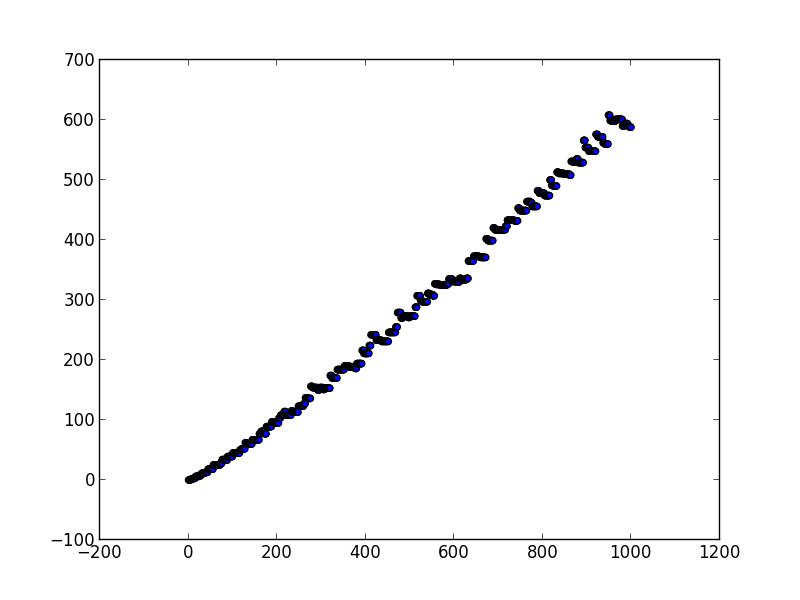
\includegraphics[width=0.4\linewidth]{TimeUntilStabilizeWithOnePeak}\label{fig:case1}} \qquad
\subfigure[Global earthquakes until stable. Horizontal axis is $n$ and vertical axis is the number of global earthquakes divided by $n$]{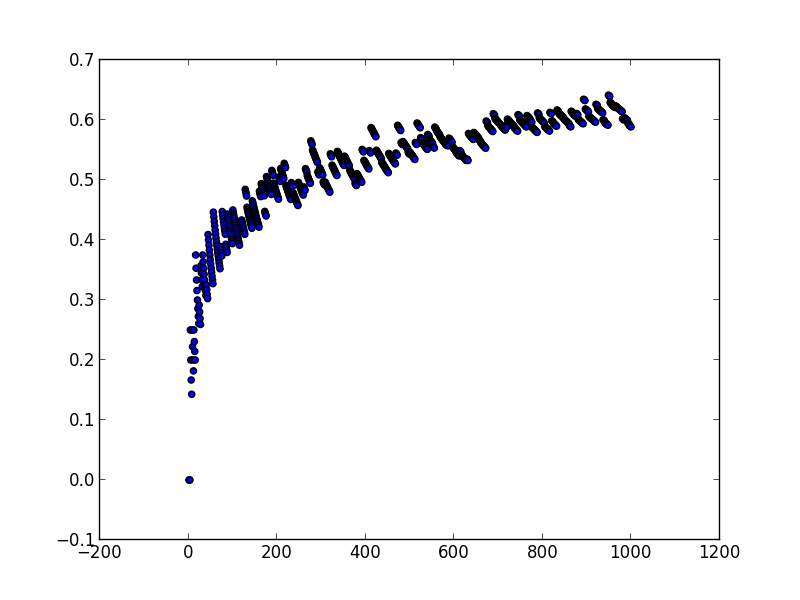
\includegraphics[width=0.4\linewidth]{Timeuntilstabledividedbyn}\label{fig:case2}}
\caption{Number of global earthquakes until stability}
\label{fig:growthofT}
\end{figure}
By looking at Figure~\ref{fig:growthofT} it seems that $T(n) = \Theta(n\log n)$. Our strategy to show a lower bound on $T(n)$ by giving a lower bound on $T'(n)$ seems to be the correct approach, since by experimental evidence (see Figure~\ref{fig:growthofT'}, we believe that $T'(n) = \Theta(n\log n)$.

\begin{figure}[!ht]
\centering
\subfigure[Local earthquakes of center until stable. Horizontal axis is $n$ and vertical axis is the number of local earthquakes]{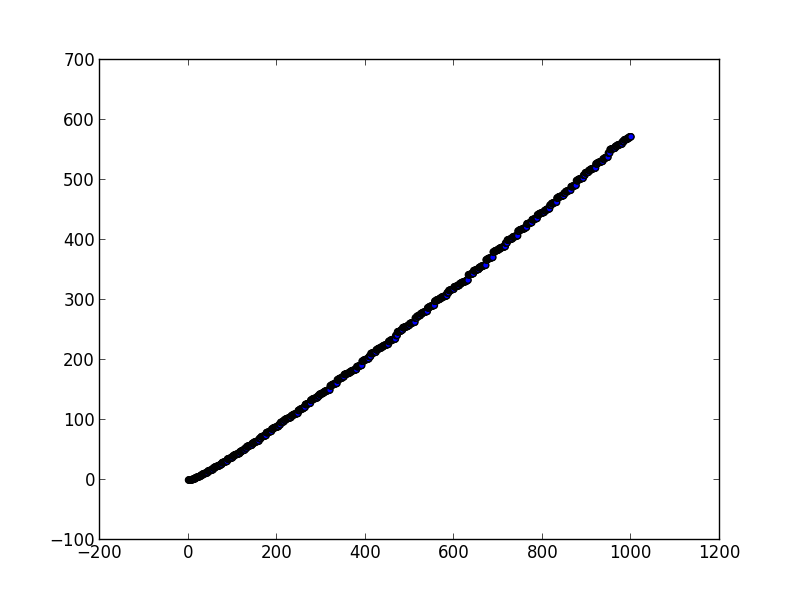
\includegraphics[width=0.4\linewidth]{centerearthquakes}\label{fig:case1}} \qquad
\subfigure[Local earthquakes of center until stable. Horizontal axis is $n$ and vertical axis is the number of local earthquakes divided by $n$]{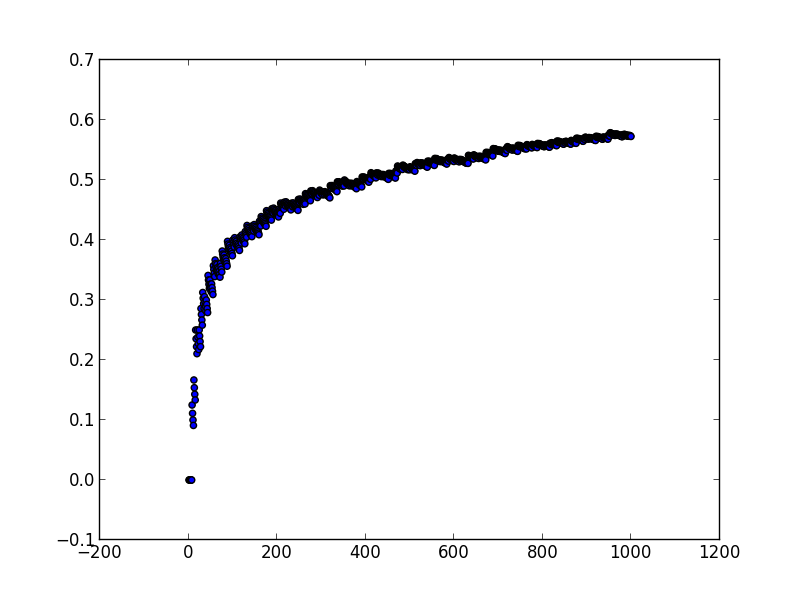
\includegraphics[width=0.4\linewidth]{centerearthquakesdividedbyn}\label{fig:case2}}
\caption{Number of local earthquakes in center until stability}
\label{fig:growthofT'}
\end{figure}



\section{Board Variants: $n$-Trees}
\label{Board Variants: n-Trees}
\emph{written by Perry Kleinhenz, edited by Fermi Ma and Erik Waingarten.}\\

Consider a semi-infinite $n$-tree. That is the graph with a parent node which has $n$ unique children. Those children each have $n$ unique children and so on. 

We can join two semi infinite $n$-trees by an edge connecting their parent nodes. This forms a graph where every vertex has $n+1$ neighbors. We would like to adapt our description of chips and earthquakes to this graph. 

\begin{definition} We define a coordinate system for our graph, with the following rules:
\begin{enumerate}
	\item $(0,0)$ and $(1,0)$ are valid coordinates and refer to the two parent nodes.
	\item $(a,b)$ is a valid coordinate for $a<0$ if $0<b \leq n^{|a|}$
	\item $(a,b)$ is a valid coordinate for $a>1$ if $0<b \leq n^{|a-1|}$
\end{enumerate}
We define the set of all valid coordinates $G_n$ as 
\begin{equation}
G_n := \{ (a,b) \in \mathbb{Z} \times \mathbb{Z} ; (a,b) \text{ obey the rules above}\}
\end{equation}
\end{definition}

\begin{definition}
We define a tree to be a map from the set of valid coordinates to the nonnegative integers, that is 
\begin{equation}
f:  G\rightarrow \mathbb{Z}_{\geq 0}
\end{equation}
We write $\mathcal{T}_n$ to refer to the set of all joined $n$-tree's 
\end{definition}

\begin{definition}
\label{bigearthquakedeftree}
We define the global earthquake operator as  as a map from the set of all $n$ trees to the set of all $n$ trees and write $GE_T: \mathcal{T}_n \rightarrow \mathcal{T}_n$. 
It transforms all of the nodes on the tree with the following rule.
\begin{equation}
GE_T(f(x,y)) = f(x,y) - (n+1)[[f(x,y) \geq n+1]] + [[f(x-k,y_0) \geq n+1]] +  \sum_{i=1}^{n} [[f(x-k,y_i) \geq n+1]] 
\end{equation} 
where $k$ is defined as 
\begin{equation}
k = \begin{cases}
1 \text{ if } x\leq 0 \\
-1 \text{ if } x \geq 1
\end{cases}
\end{equation}
and $(x-k, y_j)$ refers to the $j$th child of $(x,y)$ and $[[A]]$ is defined as 
\begin{equation}
[[A]] = 
\begin{cases} 
1 \text{ if } A \text{ is true} \\ 
0 \text{ if } A  \text{ is false}
 \end{cases}.
\end{equation}
\end{definition}

\begin{definition}
 We define the local earthquake operator as a map from the set of all $n$-trees to the set of all $n$-trees and write $LE_T: \mathcal{T}_n \rightarrow \mathcal{T}_n$.
It selects one valid node $(x,y)$ with $f(x,y) \geq n+1$ and transforms it and all of its neighbors with the following rule: 
\begin{align*}
LE_T( f( x, y ) ) = f( x , y )-n-1 \\
LE_T( f( x + k, y)) = f( x + k, y )+1 \\
LE_T( f(x-k, y_i) ) = f(x-k, y_j )+1 \\
\end{align*}
where $k$ is as defined above and $(x-k, y_j)$ refers to the $j$th child of $(x,y)$
and leaves all other squares unchanged.
\end{definition}

\begin{definition}
We say that a $n$-Tree is stable if its values are strictly less than $n+1$. This is equivalent to both of the earthquake maps having no effect on the board. 
\end{definition}

\begin{definition} 
We say that a board is finite if the total number of chips on it is finite. That is a board $f$ is finite if the sum
\begin{equation}
S= \sum_{(x,y) \in G_n} f(x,y) 
\end{equation}
is finite. 
We denote the set of finite boards as $\mathcal{T}_n^f$.
\end{definition}

As it turns out we can use a  method of proof nearly identical to the standard board case to show that the state of a tree under this process can never cycle.

We once again define a potential function 
\begin{definition} Let $\Phi: \mathcal{T}_n^f \rightarrow \mathbb{Z}_{\geq 0}$ be the  function
\begin{equation}
\Phi(f) = \sum_{(x,y) \in G_n} f(x,y)(|x|)^2
\end{equation}
Note that this is well defined for trees which contain a finite number of chips. 
\end{definition} 

\begin{lemma}
If $LE_T(f) \neq f$, then $LE_T^n(f) \neq f$ for all $n > 0$.
\end{lemma}

\begin{proof}
We will show that  if $LE$ acts on a board nontrivially then $\Phi(LE(f))$ will be strictly larger. That is  
\begin{equation}
LE(f) \neq f \Rightarrow \Phi(LE(f)) > \Phi(f)
\end{equation}


We can evaluate $\Phi(LE(f)) - \Phi(f)$.
\begin{align}
\Phi(LE_T(f))-\Phi(f) = \sum_{(x,y) \in G_n} LE_T(f)(x,y)(x)^2 - \sum_{(x,y) \in G_n} f(x,y)(x)^2 
\end{align}
Only one node call it $(x_0,y_0)$ and its neighbors are affected. Therefore the above expression simplifies to
\begin{align*}
\Phi(LE_T(f)-\Phi(f) = LE_T( f(x_0,y_0) )* (x_0)^2 + LE_T( (f(x_0+k, y_0) )* (|x_0+k|)^2 \\
+ \sum_{i} LE_T( f(x_0-k, y_i) ) * (|x_0-k|)^2 \\
= -(n+1)*(|x_0|)^2 + (|x_0+k)^2 + n (|x_0-k|)^2 \\
\geq-(n+1)*(|x_0|)^2 + (|x_0|-1)^2 + n (|x_0|+1)^2
= -nx^2-x^2+x^2-2|x|+1+n(x^2+2|x|+1) \\
= 2x(n-1)+n+1 > 0
\end{align*}
Where $(x_0-k,y_i)$ refers to the $j$th child of $(x_0,y_0)$ and $k$ is as defined in Definition \ref{bigearthquakedeftree}.
\end{proof}

\begin{lemma}
If $GE_T(f) \neq f$, then $GE_T^n(f) \neq f$ for all $n > 0$.
\end{lemma}

\begin{proof}
We will show that 
\begin{equation}
GE_T(f) \neq f \Rightarrow \Phi(GE_T(f)) > \Phi(f)
\end{equation}
This means that if there is an earthquake that changes things, then $\Phi(f)$ increases, which means that if $E(f) \neq f$, then for all $N > 0$, $E^N(f) \neq f$, or that you never return to your original state.

We can evaluate $\Phi(GE_T(f)) - \Phi(f)$.
\begin{align}
\Phi(GE_T(f))-\Phi(f) = \sum_{(x,y) \in G_n} GE_T(f)(x,y)(|x|)^2 - \sum_{(x,y) \in G_n} f(x,y)(|x|)^2 
\end{align}
Let $A$ be the set of active locations, or locations with $f(x,y) \geq (n+1)$, which is non-empty by assumption. 
\begin{align*}
\Phi(GE_T(f)) - \Phi(f) =  \sum_{(x,y) \in A}  GE_T(f(x,y))x^2 + GE_T(f(x+k,y))(|x+k|)^2 + \\
\sum_{i} \left( GE_T(f(x-k,y_i))(|x-k|)^2 \right) -f(x,y)x^2 +f(x+k,y) (|x+k|)^2 +  \sum_{i} \left ( f(x-k,y_i) (|x-k|)^2 \right)  \\
=\sum_{(x,y) \in A} -(n+1)x^2 + (|x+k|)^2 + n(|x-k|)^2 
\end{align*}
Where $(x-k,y_i)$ refers to the $j$th child of $(x,y)$ and $k$ is as defined in Definition \ref{bigearthquakedeftree}. We note that each term in this sum is positive by our proof of the lemma for local earthquakes and so the sum itself must be positive. That is 
\begin{equation}
\Phi(GE_T(f)) - \Phi(f) > 0
\end{equation}

\end{proof}

\begin{lemma}
\label{finiteextensiontree}
Suppose $\sum_{x,y} f(x,y) = S$, and all chips are between the levels $[x_l, x_h]$. Then $GE_T^m(f)$ and $LE_T^m(f)$ only contain chips within the range $[x_l - 2S, x_h + 2S]$ for all $m$.
\end{lemma}

\begin{proof}
It is obvious that a board with $S$ chips on level $l<0$ will have a lower $X_{min}$ than a board with $S$ chips on level 0, and the analogous statement for $X_{max}$ holds as well. 

Now as a very crude lower bound we know that $S$ chips on a single node at level $l<0$ will have an $X_{min}$ no lower than $l-2S$ as there must be at least one chip on every other level, as chips only move one level at a time. 

If we take any other arrangement of $S$ chips, with $X_{min}=l$ but not all $S$ chips are on a single node. We know that $X_{min}$ for this board is bounded below by $l-2S$. In order to have an $X_{min}$ below this at some point in time it would be possible to have $S$ chips on the same node on level $l$. But this cannot occur because in order to move a chip down a level, one chip must move up a level. Therefore if $X_{min}=x_l$, both $GE_T^m(f)$ and $LE_T^m(f)$ do not contain chips below level $x_l -2S$.

An analogous argument shows that if $X_{max}=x_h$, both $GE_T^m(f)$ and $LE_T^m(f)$ do not contain chips above level $x_h+2S$.
\end{proof}

So now we are ready to prove the theorem that all finite boards will reach a stable state. 

\begin{proof}
(of Theorem~\ref{finitestability}) Suppose $f \in \mathcal{B}$ is a finite board, so $\sum_{x,y} f(x,y) = S$, and suppose all chips lie between levels  $[x_l, x_h]$. Then by Lemma ~\ref{finiteextensiontree}, we have that for all $m$ all chips in $GE_T^m(f)$ and $LE_T^m(f)$ will lie in $R = [x_l - 2S, x_h + 2S]$

We have restricted the size of the board to be finite, and the number of chips that can be placed on the board to be finite. 
Thus the total number of ways that the chips can be arranged on the board is finite. 
In particular there are fewer than $(x_h - x_l+1 + 4 S)$ levels and there are at most 
\begin{equation}
n^d,
\end{equation}
nodes at each level, where $d= \max(x_h, |x_l|)$. So there are at most 
\begin{equation}
N:=(x_h - x_l+1 + 4 S)n^d
\end{equation}
nodes that are potentially occupied. Therefore there are at most 
\begin{equation}
\binom{N+S-1}{N-1}
\end{equation}
possible boards $b \in \mathcal{T}_n^f$ that satisfy this. We know that there are no cycles in the states, so there must be an $0 \leq N < \binom{N+S-1}{N-1}$ such that $E^N(f) = E^{N+m}(f)$ for all $m \geq 0$.
\end{proof}


\section{Computing with Chips}
\label{Computing with Chips}

\emph{Written by Erik Waingarten, edited by Fermi Ma and Perry Kleinhenz.}

In this section, we show how we can compute different Boolean functions using the poker chip board and the earthquake operator.

A Boolean input is a number in $\{0,1\}$, and a Boolean function is a function that takes $k$ Boolean inputs and outputs a number in $\{0,1\}$. A simple Boolean function is the AND function that takes in 2 Boolean inputs, and returns a 1 if and only if both the input values are set to 1. Another Boolean function is the OR function, that takes in 2 Boolean inputs, and returns a 0 if and only if both input values are set to 0. If 0 is associated with ``false" and 1 is associated with '``true", then the AND function returns ``true" if both inputs are ``true", and the OR function returns ``true" if at least one input is true. More complicated Boolean functions can be made with more than 2 inputs and compositions of these inputs. Denoting an AND with $\vee$ an OR with $\wedge$, we can construct composite functions such as $b_1 \wedge (b_2 \vee b_3)$. 

Boolean circuits are formed by using wires that transmit 0's and 1's, and feeding them through various \emph{gates}. For example, a wire carrying a 0 and a wire carrying a 1 can be fed through an OR gate, which will ``output" a wire carrying a 1. In this section, we construct circuits using the poker chips board that use AND an OR gates. 

\subsection{Model of Computation}

Our model of computation is as follows: we assume a finite board with finitely many chips. The inputs are designated by each two squares, one apart one is the ``clock" square and other the bit square. Likewise, the outputs each have a ``clock" square and a bit square. The ``clock" squares are set the value 4 and the bit squres are set to 4 if they are 1 and 0 otherwise. A computation is done by a series of earthquakes, when an output has the clock square active, then the bit square is read, and that output bit is considered read. 

\subsection{Example}

A simple example is given by a board that computes the identity.

\[ \begin{array}{cccccc} 0 & 0 & 0 & 0 & 0 & 0 \\
				     4_c & 3 & 3 & 3 & 3 & 3_e \\
				     0 & 0 & 0 & 0 & 0 & 0 \\
				     i  & 3 & 3 & 3 & 3 & 3_o \\
				     0 & 0 & 0 & 0 & 0 & 0 \end{array} \]
Where the subscript $c$ indicates the clock, the subscript $e$ indicates the output clock square. $i$ indicates the bit square, and $o$ indicates the output bit. 

One can see that $e$ will become active after 5 earthquakes since it will take that many earthquakes for $c$ to reach $e$. Also, if $i$ is initially inactive, then $o$ will be inactive, and if $i$ is active, then $o$ will be active. Therefore, we can compute the identity. 

This circuit also shows how to make a ``wire" in the circuit. We will represent a wire as two parralel arrows, one containing the clock path and the other carrying the input. 

\subsection{Turner}

Turning is non trivial, we must guarantee that we can turn a signal and align the timinings of the inputs and outputs in the clock so that they have the same distance. this is a counter-clockwise turn where $c$ denotes the clock, $i$ is the input bit, then $e$ is the output clock and $o$ is the output bit.

\[ \begin{array}{cccccc} 0 & 0 & e & 0 & o \\
				     0 & 3 & 2 & 0 & 3 \\
			            0 & 2 & 3 & 0 & 3 \\
				    0 & 3 & 2 & 0 & 3 \\
				    0 & 2 & 3 & 0 & 3 \\
				    c & 3 & 3 & 0 & 3 \\
				    0 & 0 & 0 & 0 & 3 \\
				    i & 3 & 3 & 3 & 3 \end{array} \]	
Since the clock snakes along the path while $i$ takes the shorter path. 
Likewise, we can perform a clockwise path by making $i$ snakes while the clock takes a straight path. 

\subsection{Synchronize}

We can synchronize the inputs so that the input signal waits for the clock to arrive. This can be simply done with the following board configuration:
\[ \begin{array}{cccccccc} c & 3 & 3 & 3 & 3 & 3 & 3 & 0 \\
					 0 & 0 & 0 & 0 & 3 & 0 & 3 & 0 \\
					 i  & 3 & 3 & 3 & 1 & 3 & 3 & 3 \\
					 0 & 0 & 0 & 0 & 3 & 0 & 0 & 3 \\
					 0 & 0 & 0 & 0 & o & 0 & e & 3 \end{array} \]
Note that the path from $i$ to $o$ is 6 units long, while the path from clock is 12 unit long. $i$ waits for the clock since it needs the signal from $c$ from two sides to activate the 1 in the path from $i$ to $o$.

The fact that we have a synchronizer means that the model of computation is equivalent to one where there is only one clock for all input bits. 

\subsection{Boolean circuits}

Now we can show how to compute some basic boolean functions and since we have turns and synchronizers, we can assume that we have synchronized the inputs already. The following can compute the AND of two inputs. 

\[ \begin{array}{cccccccc}    &    & c_1&   &  i_1 &     &  \\
					   &    & 3   & 2 &  3    &    &  \\
					   &    &    & 3 &    & 3 & c_2 \\
					o & 3 & 3 & 2 & 3 & 2 & 	    \\
					   &    &    &    &    & 3 & i_2 \end{array} \]
Where we can make the $c_1$ and $c_2$ snake around before hand to guarantee that they are synchronized, and then we can make $c_1$ snake around so that it becomes the clock of the output. So in this case, $o = i_1$ AND $i_2$.

Similarly, we can compute the OR of two circuits with a very simple modification:
\[ \begin{array}{cccccccc}    &    & c_1&   &  i_1 &     &  \\
					   &    & 3   & 2 &  3    &    &  \\
					   &    &    & 3 &    & 3 & c_2 \\
					o & 3 & 3 & 3 & 3 & 2 & 	    \\
					   &    &    &    &    & 3 & i_2 \end{array} \]
And we can do a similar set up to synchronize the clocks. 

So currently, we can compute any boolean circuit which can be drawn in a planar graph with only ANDs and ORs. So the question is whether we can compute the NOT? We argue that this is not possible. 

\begin{theorem}
There does not exists any board configuration which computes the NOT operator in the above model of computation.
\end{theorem}

\begin{proof}
Suppose we have a board configuration $B$ with input squares $c$, $i$ and output squares $e, o$ that computes the NOT function. Then we can make another board $B'$ that synchronizes the final clock with the input so that we do not need to worry about timing of the clock. That is, we can guarantee that if $o$ is active, then $o$ is active at the same time $e$ is active.

Now lets make $B'$ an infinite board by putting 0s on the sides. So we have a finite board with finitely many chips. Let $S_{c_0i_0}$ be the set of squares which were active (had an earthquake affect them) during the execution of $B$ with the input value $i = i_0$ and $c = c_0$. 

The first claim to make is that $S_{c_0i_0} \subset S_{c_1i_1}$ if $c_0 \leq c_1$ and $i_0 \leq i_1$. This is clearly true since the order of redistribution does not matter. In fact, we can do the earthquakes by first doing the earthquakes on $c$ and $i$ until the value decreases past $c_0$ and $i_0$, then simulate the computation of $c = c_0$ and $i = i_0$ with local earthquakes.

However, this arises in a contradiction, since $o \in S_{10}$ but $o \notin S_{11}$. Therefore, computing NOT with a board is not possible.
\end{proof}

What does this mean? Well, in particular, it means that we cannot do much. In particular, we can't add, since $x + 1$ will act as the NOT operator on the lowest order bit. We can only compute boolean circuits in planar graphs. 


\end{document}
